\section{Introduction}

The economic question is not only whether artificial intelligence can perform
tasks currently done by workers. It is also whether AI can perform the research
that produces better AI. When current AI capability determines the productivity
of compute used both in final production and in AI research, a familiar
substitution problem also creates a dynamic feedback. Following the useful
distinction in \citet{davidsonetal2026}, higher capability operates through two
loops. The technological loop raises the services produced by research compute;
the economic loop raises output and therefore the resources that can be devoted
to accumulation and research. Higher capability also lowers the resource cost of
a unit of AI service. The conditions under which this
feedback can settle into balanced growth or enter an accelerating branch depend
on substitution possibilities in both sectors, the strength of the resulting
feedback, and the branch that is reached.

This paper studies that feedback in a general-equilibrium growth model. Raw
compute has two uses. Inference compute is transformed by current AI capability
into services used in final production. AI R\&D compute---called research compute
below---is transformed by the same capability into automated research services.
Human researchers and automated research services are combined with a CES
technology to improve AI capability.
An integrated monopolist sells production services to final-good firms and uses
automated research services internally. The representative household owns capital
and the developer, supplies labor, and chooses consumption. Population grows
exogenously.

Research substitution and research scale are separate. The elasticity
\(\sigma_{HM}\) governs the response of the input mix to relative prices, whereas
\(0<\eta<1\) imposes decreasing returns to a proportional expansion of current
research inputs, holding capability fixed. The boundary \(\eta=1\) is substantive,
not a normalization. The baseline imposes the stronger restriction
\(\eta<\alpha\). Proposition \ref{prop:axm-research-burst} shows why. For all
positive CES elasticities, on any fixed horizon with regular positive price and
quantity paths, let \(S\) denote
total research expenditure. Capability is at most of order
\(1+S^{\eta/(1-\eta)}\), and optimized operating profit implies the bound
\[
 J_T\leq C_0+C_1S^{\eta(1-\alpha)/[\alpha(1-\eta)]}-cS.
\]
The exponent is below one exactly when \(\eta<\alpha\). The truncated
developer objective is then coercive over all nonnegative research policies,
and its supremum is finite. If both CES nests permit gross substitution and
\(\eta>\alpha\), a fixed-duration expansion of research compute makes the
truncated value unbounded. Extending each policy
with zero controls after the truncation date also makes the corresponding
infinite-horizon developer value unbounded under the stated extension conditions.
At equality, coefficients rather than exponents determine the leading term of
this family, and the boundary is not fully characterized. With
\((\alpha,\eta)=(0.33,0.20)\), the exponent equals 0.5076. This result does
not establish compactness of the control set, attainment of the supremum,
global optimality, infinite-horizon well-posedness, or equilibrium existence.

The distinction between raw compute and the services produced by compute is
central. A unit of compute is not a unit of intelligence. Current capability
determines what a given unit of hardware, energy, and datacenter time can produce.
We therefore write production services as the product of capability and inference
compute, and automated research services as the product of capability and research
compute. This capability-times-compute architecture is the one-capability analogue
of the AI-service accounting in \citet{davidsonetal2026}. It is also informed by
the richer distinction between inference output, training activity, algorithms,
and model capital in \citet{korinekmckelvey2026}. Our reduction is substantive:
one stock \(A\) combines model quality and algorithmic efficiency and augments
both uses of compute. Our term research compute corresponds to their broad
training-and-R\&D compute category. It includes pretraining, post-training,
experimentation, synthetic-data generation, automated algorithmic search, and
compute used by AI systems engaged in research.

The model deliberately excludes a separate power of the capability stock from its
baseline research technology. Better AI affects research only by making research
compute more productive. In the terminology of \citet{davidsonetal2026}, the
parameter governing returns to the current scale of research and the parameter
governing intertemporal idea difficulty are distinct. Our \(\eta\) is the former;
the baseline imposes \(b=1\) on the latter. A term such as \(A^{1-b}\) could make
that second margin free: holding the effective-research index fixed, any \(b>0\)
introduces the familiar ideas-getting-harder force in the growth rate of capability,
while \(1-b>0\) also gives the stock a positive level effect on \(\dot A\)
\citep{jones1995,davidsonetal2026}. Setting \(b=1\) removes this separate
level-stock term and isolates the feedback carried by automated research services.

\subsection{Empirical motivation}

Available data do not measure the objects at the center of the research block:
the relative use and contribution of human researchers and automated research
services. They do, however, provide
separate measures of raw compute, electricity use, and quality-adjusted AI output.
In the data cited below, both the physical resources devoted to AI and the
services obtained from those resources expand rapidly, with quality-adjusted
output rising faster. These measures motivate the distinction between raw compute
and AI services; they do not identify either substitution elasticity.

\citet{korinekmckelvey2026} estimate that U.S. AI compute expenditure rose from
\$36.9 billion in 2023 to \$219.2 billion in 2025, while raw compute capacity rose
from 1.09 million to 10.7 million H100-equivalent units of compute capacity, a measure normalized
to the computing capacity of an NVIDIA H100 accelerator. Over the same two years,
their quality-adjusted inference and training indexes increased by factors
of approximately 1,502 and 78. The quality-adjusted series are model-based
estimates assembled from sparse data and allocation assumptions, not
national-account aggregates. Their relevance here is conceptual: more compute and
more services per unit of compute are distinct margins.

\begin{figure}[t]
\centering
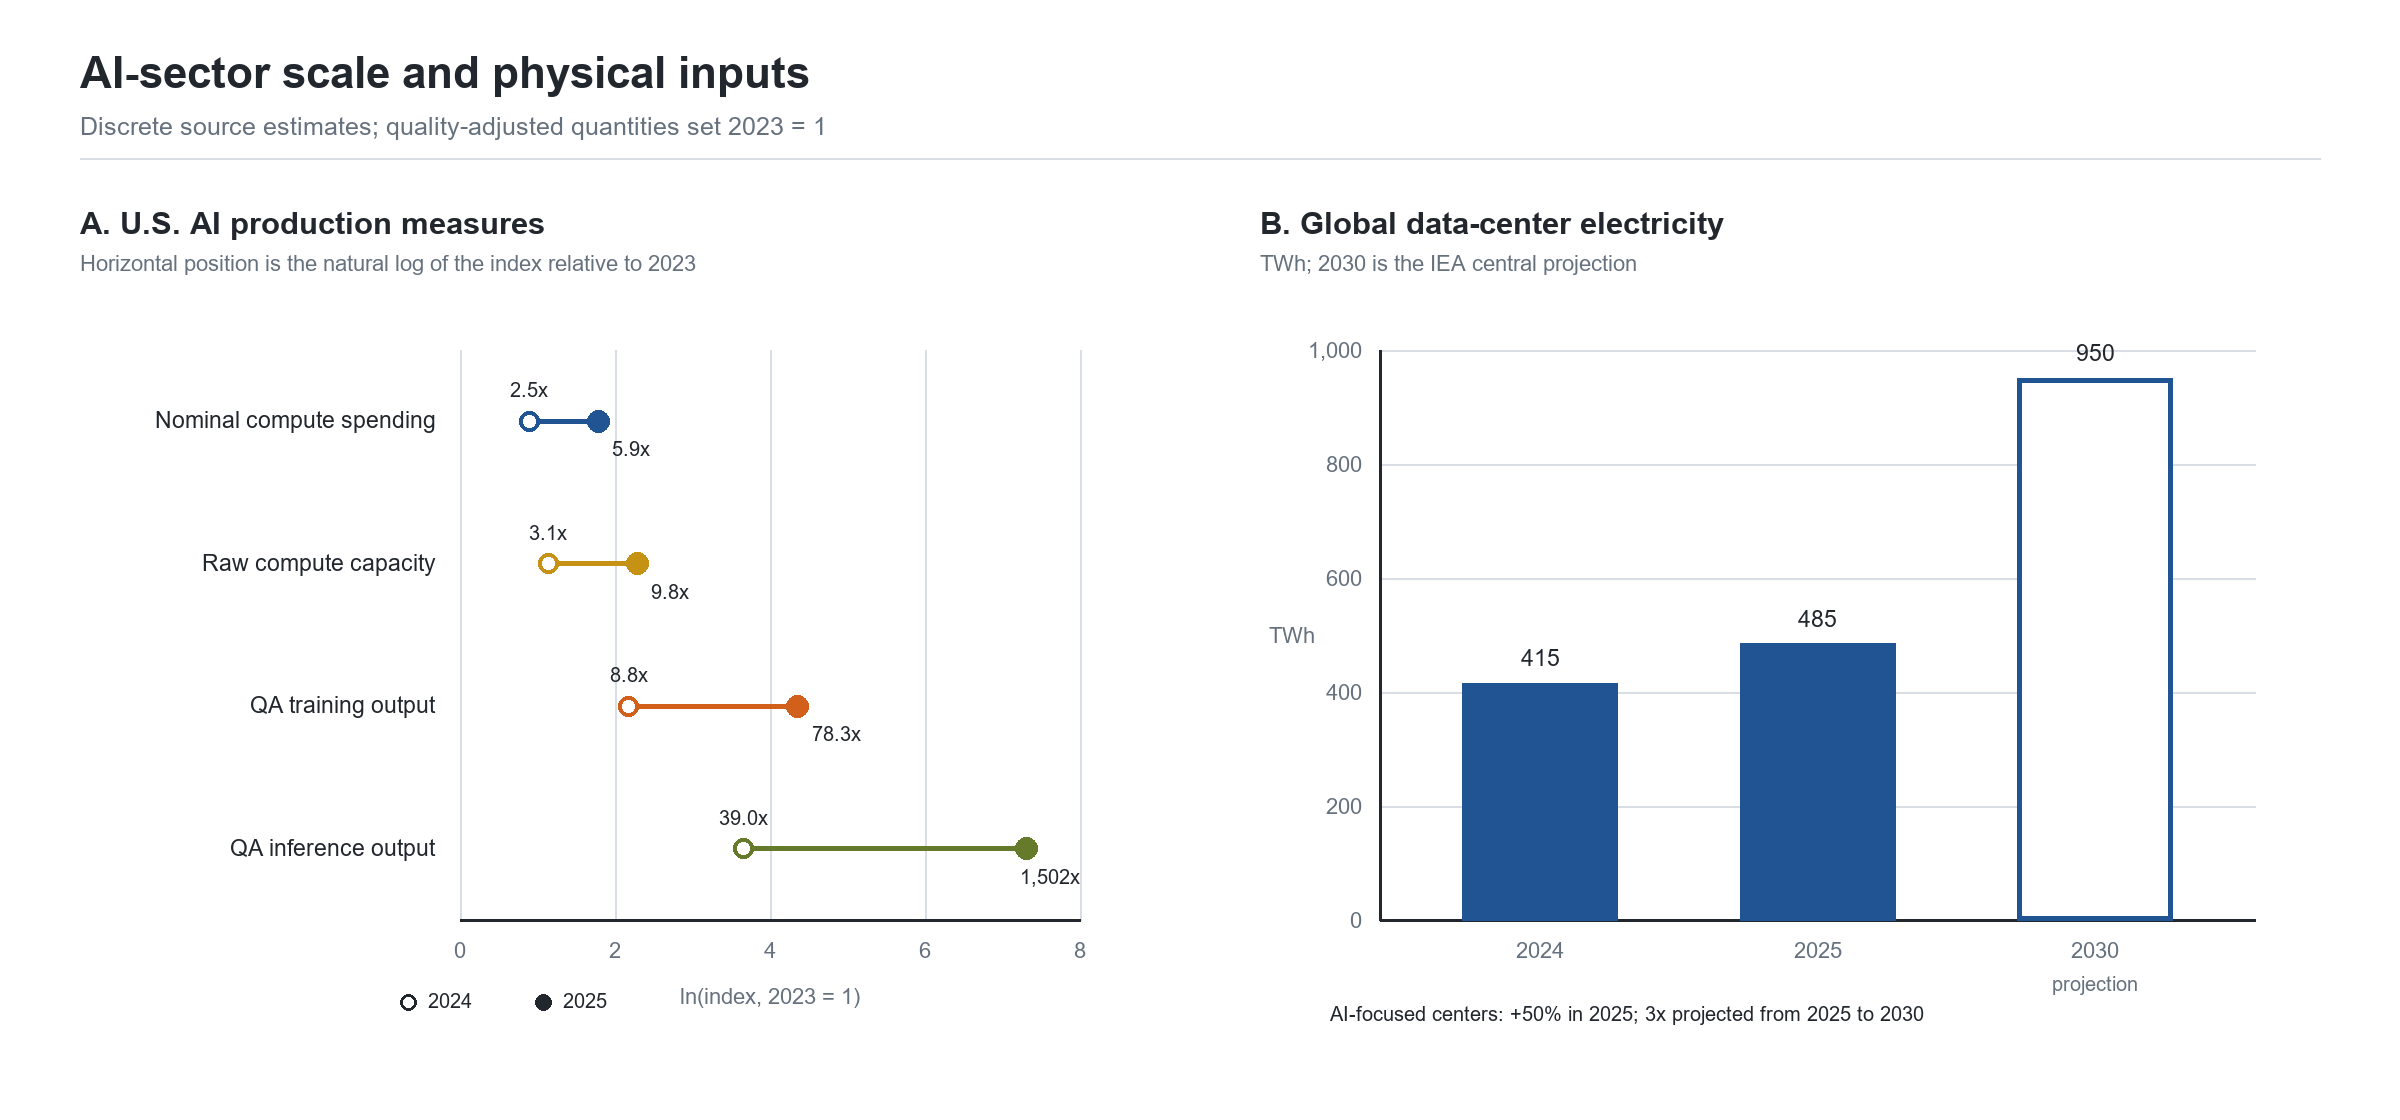
\includegraphics[width=\textwidth]{figures/empirical_ai_scale.png}
\caption{AI-sector scale and physical inputs. Panel A reports U.S. estimates for
2024 and 2025 relative to 2023; horizontal positions use natural logarithms because
the quality-adjusted quantities span several orders of magnitude. Panel B reports
IEA estimates of global data-center electricity use in 2024 and 2025 and its central
projection for 2030. Sources: \citet{korinekmckelvey2026}, \citet{iea2025}, and
\citet{iea2026}.}
\label{fig:axm-empirical-scale}
\end{figure}

Compute nevertheless remains a real resource. The International Energy Agency
estimates that global data-center electricity use rose from 415 TWh in 2024 to
485 TWh in 2025, and it projects approximately 950 TWh in 2030
\citep{iea2025,iea2026}. Normalizing the
common unit cost of inference and research compute therefore changes units; it
does not remove compute from the resource constraint.

Evidence closest to AI research automation comes from controlled evaluations. In
the original RE-Bench study, human experts with a 32-hour budget achieved almost
twice the average score of the best AI agent on machine-learning
research-engineering tasks \citep{metrrebench2024}. In a later evaluation on a
five-task subset, aggregating shorter Claude 3.7 runs to 32 hours produced a score
comparable to the median human score at eight hours \citep{metrclaude2025}.
These five tasks have unusually clear objectives and rapid feedback, and the model,
surrounding agent software and tools, tasks, and time budgets differ. The results
are therefore neither a comparable time series nor a measure of substitution in
real-world AI research. They
motivate the possibility of substitution in AI research without measuring
\(H/(AM)\) or \(\sigma_{HM}\).

The numerical exercises below are therefore scenarios rather than forecasts. The
evidence motivates the distinction between raw compute and service flows and the
two uses of compute, but it does not calibrate the feedback strength or the
conditions under which the economy reaches the accelerating branch.

\subsection{Results and contribution}

The analysis separates three regimes according to the elasticity of substitution
between labor and AI services in final production. When the elasticity is below
one, an interior complementarity limit satisfying the regularity conditions in
Proposition~\ref{prop:axm-complements} has a finite ratio of AI services to
production labor. Final output then becomes asymptotically proportional to a
Cobb--Douglas function of capital and production labor. On any finite-rate
balanced-growth path that satisfies the stated conditions and keeps production
labor at a positive population share, output per capita is constant. The audited
finite-horizon candidate paths make the distinction from research automation
visible: capability keeps growing in both reported complementarity cases, and
with substitutable research the automated research-expenditure share approaches
one. Over the same transition, output per person, consumption per person, and the
real wage move toward their conditional constant limits, while labor retains a
positive income share. At unit elasticity, the paper
derives the growth rates and resource shares of balanced-growth candidates. An
asymptotically automated research sector places greater weight on the feedback
from capability to both production and research and therefore tightens the
condition for positive balanced growth. When the final-production elasticity
exceeds one and AI services asymptotically dominate the labor--AI composite,
unbounded capability raises \(Y/K\) and the net interest rate without bound. A finite-rate
balanced-growth path is then impossible.

For the regime with gross substitution in both final production and AI research,
the paper goes beyond this nonexistence result.
It characterizes a conditional AI-dominated limiting branch of the necessary
conditions on which output, capital, consumption, and capability accelerate. The characterization assumes
that the path remains interior, converges to the postulated ratios, and satisfies
the monopoly second-order condition. Under those conditions,
aggregate labor income as a share of output tends to zero, while the real wage
rises when the smaller of the two substitution elasticities is below an explicit
threshold and falls when it is above that threshold. The distinction between labor income's
share of output and the wage level is economically important: a factor may
receive a vanishing fraction of an economy that is expanding even faster.

The complementarity and unit-elasticity computations solve the same dated
equilibrium system under the capability law used in the paper. The two reported
unit-elasticity parameterizations also satisfy the sufficient
concavity restrictions in Proposition \ref{prop:axm-equilibrium-sufficiency}.
Their numerical path approximations solve the household Euler equation, the developer's
research first-order conditions and costate equation, the monopoly pricing
condition, both market-clearing conditions, and the two laws of motion. The
simulations are used to illustrate propositions, not to replace them. The reported
paths are rejected unless all dated static, first-order, market, and dynamic
residuals are small and the monopoly second-order margin is positive. Finite
terminal conditions approximate, but do not prove, the infinite-horizon
transversality limits.

For gross substitution in final production, a separate free-boundary calculation
solves the necessary conditions up to successively larger values of \(Y/K\).
The resulting paths converge on common pre-singular intervals and their estimated
singularity dates converge. This is evidence for the conditional accelerating
branch, but not a proof of its global intertemporal optimality, reachability from
arbitrary initial states, or continuation beyond the finite-time boundary.

The closest analytical benchmark is \citet{davidsonetal2026}, who already
combine nonrival AI capability with rival compute and distinguish technological
from economic feedback in a multitechnology innovation network. This paper embeds
a one-capability version of that architecture in a decentralized Ramsey economy
with an integrated monopolist. Its contribution is to determine inference and
research compute, production and research labor, saving, prices, and factor shares
jointly rather than fixing the relevant allocation shares. The two CES margins
make the local link weights endogenous equilibrium objects determined jointly by
relative prices and allocations. In the
unit-elasticity regime, the balanced-growth denominator becomes the scalar analogue
of Davidson et al.'s feedback-matrix condition. In the conditional AI-dominated
limit, the model also derives an explicit threshold separating rising from falling
wages: the relevant elasticity is the smaller of the substitution elasticities in
final production and AI research. This result does not infer wage behavior from
labor income's share of output.
